\documentclass[usenames,dvipsnames]{beamer}
\usepackage{pgfpages}
\setbeameroption{show notes on second screen=right}
\setbeamertemplate{note page}[plain]
\usepackage{tikz}
\usetikzlibrary{cd}
\usepackage{catchfilebetweentags}
\usepackage{amssymb}
\usepackage{turnstile}
\usepackage{bbm}
\usepackage[greek, english]{babel}
\usepackage{MnSymbol}
\usepackage{stmaryrd}
\usepackage{csquotes}
\newcommand\doubleplus{+\kern-1.3ex+\kern0.8ex}
\newcommand\mdoubleplus{\ensuremath{\mathbin{+\mkern-8mu+}}}
\makeatletter
\newcommand\incircbin
{%
  \mathpalette\@incircbin
}
\newcommand\@incircbin[2]
{%
  \mathbin%
  {%
    \ooalign{\hidewidth$#1#2$\hidewidth\crcr$#1\bigcirc$}%
  }%
}
\newcommand{\oeq}{\ensuremath{\incircbin{=}}}
\makeatother
\usepackage{ucs}
\DeclareUnicodeCharacter{8759}{\ensuremath{\squaredots}}
\DeclareUnicodeCharacter{951}{\textgreek{\texteta}}
\DeclareUnicodeCharacter{737}{\ensuremath{^\text{l}}}
\DeclareUnicodeCharacter{691}{\ensuremath{^\text{r}}}
\DeclareUnicodeCharacter{7523}{\ensuremath{_\text{r}}}
\DeclareUnicodeCharacter{8718}{\ensuremath{\blacksquare}}
\DeclareUnicodeCharacter{957}{\textgreek{\textnu}}
\DeclareUnicodeCharacter{961}{\textgreek{\textrho}}
\DeclareUnicodeCharacter{929}{\textgreek{\textRho}}
\DeclareUnicodeCharacter{954}{\textgreek{\textkappa}}
\DeclareUnicodeCharacter{10214}{\ensuremath{\lsem}}
\DeclareUnicodeCharacter{10215}{\ensuremath{\rsem}}
\DeclareUnicodeCharacter{8857}{\mdoubleplus}
\DeclareUnicodeCharacter{8860}{\oeq}
\DeclareUnicodeCharacter{9043}{\ensuremath{\triangle}}
\DeclareUnicodeCharacter{928}{\textgreek{\textPi}}
\DeclareUnicodeCharacter{922}{\textgreek{\textKappa}}
\DeclareUnicodeCharacter{931}{\textgreek{\textSigma}}
\DeclareUnicodeCharacter{916}{\textgreek{\textDelta}}
\DeclareUnicodeCharacter{8779}{\ensuremath{\backtriplesim}}
\DeclareUnicodeCharacter{8799}{\ensuremath{\stackrel{?}{=}}}
\DeclareUnicodeCharacter{10181}{\ensuremath{\lbag}}
\DeclareUnicodeCharacter{10182}{\ensuremath{\rbag}}
\usepackage[utf8x]{inputenc}
\usepackage[T1]{fontenc}
\usepackage{autofe}
\usepackage[references]{agda}
\usepackage{bbding}
\setlength{\marginparwidth}{2cm}
\usepackage[obeyDraft]{todonotes}
\usepackage{graphicx}
\usepackage{tikz}
\usetikzlibrary{decorations.pathmorphing}
\usetikzlibrary{snakes}
\usetikzlibrary{arrows}
\usepackage{forest}
\usepackage{multicol}
\usetheme{metropolis}
\usepackage{natbib}
\usepackage{bibentry}
\usepackage[draft=false]{minted}
\usepackage{amsmath}
\usepackage{tabularx}
\metroset{block=fill}
\usepackage{adjustbox}
\title{Talking About Mathematics in a Programming Language}
\author{Donnacha Oisín Kidney}
\begin{document}
\maketitle
\tableofcontents
\bibliographystyle{plain}
\nobibliography{../horners-rule.bib}
\section{What do we want from a Language for Mathematics?}
\begin{frame}
  \frametitle{What do we want from a Language for Mathematics?}
  \note<1>{
    As it turns out, the languages we use for maths already look a little like
    programming languages.

    In designing them we encounter a lot of the same goals.
  }
  \pause
  \begin{columns}[T]
    \column{0.5\textwidth}
    \begin{block}{A \emph{Syntax} that is}
      \begin{itemize}
        \item Readable
        \item Precise
        \item Terse
      \end{itemize}
    \end{block}
    \pause
    \column{0.5\textwidth}
    \begin{block}{\emph{Semantics} that are}
      \note<3>{
        Semantics/axiomatic core
      }
      \begin{itemize}
        \item Small
        \item Powerful
        \item Consistent
      \end{itemize}
    \end{block}
  \end{columns}
  \note<3>{
    Some of these are conflicting!
  }
\end{frame}
\begin{frame}[standout]
  Why not use a Programming Language?
\end{frame}
\begin{frame}
  \frametitle{Reason 1: Because Computer-Assisted Proofs are ``Bad''}
  \note<1>{
    Aren't computer-assisted proofs bad? Inelegant? Less rigorous?
  }

  \pause
  \bibentry{appel_solution_1977}
  \note<2>{
    The famous example is the four-colour map theorem.

    First major mathematical proof which relied heavily on computer assistance.

    The problem is thus: can you colour a map, with only four colours, so that
    every border has two different colours?

    The proof effectively relied on checking a large number of different
    cases---a computer program was used to check each one.
  }
  \pause
  \begin{itemize}
  \item Non-Surveyable
    \pause
    \note<3>{
      The proof is too large for another mathematician to check its work! (that
      is, after all, why a computer was used)
    }
  \item Doesn't Provide Insight
    \pause
    \note<4>{
      This is maybe an aesthetic concern, but the prevailing attitude is that a
      non computer-assisted proof would provide a deeper understanding of the
      problem, and more general tools to be used later, rather than a simple
      statement ``yes the proposition is true'' or ``no it's false''.

      Of course, in practice, working a proof to a level where it becomes
      solvable via a computer requires insight in and of itself, but perhaps
      less insight than another method.
    }

  \item Requires Trust
    \note<5>{
      We have to believe that the program used to prove the proposition doesn't
      contain bugs!
    }
  \end{itemize}
  \pause
  Did contain bugs!
  \note<6>{
    Although they weren't critical to the correctness.
  }
\end{frame}
\begin{frame}
  \frametitle{This is Different}
  \pause
  We're looking for a core set of axioms/semantics and a syntax to talk about
  mathematics
  \note<2>{
    We're going to use PL theory to help get us there
  }
  
  \pause
  If we do it right, it should be so simple that ``even a computer could
  understand it''
  \note<3>{
    But this is incidental!

    The real work is in finding the language that works.

    Even now, most compilers for these languages are grad students!
  }


  \pause
  \begin{block}{Why would we want a computer to understand our language?}
    \pause
    \begin{itemize}
      \item So it can check our proofs! \pause
      \item So it can check our \emph{automated} proofs!
    \end{itemize}
  \end{block}

  \note<5>{
    If a machine can read your proofs, then it can \emph{check} your proofs.

    This adds a level of rigour that you just don't get with handwritten proofs.
  }
  \note<6>{
    A perfect candidate for the kinds of proofs we'd like a machine to check
    \emph{are} computer-assisted proofs.

    Remember, our language is a programming language: write the automated
    theorem prover in it, and then \emph{verify} the theorem prover in it!
  }

  \pause
  \bibentry{gonthier_formal_2008}
  \note<7>{
    Unfortunately, this is still difficult to do

    The formalized version of the four-colour theorem came out a full 29 years
    later!
  }
\end{frame}
\begin{frame}[fragile]
  \frametitle{Reason 2: Haven't We Tried This Before?}
  \note<1>{
    Fully formalizing mathematics from the ground-up has long been a goal.
    (Hilbert)

    Haven't other attempts failed?
  }
  \begin{columns}
    \column{0.5\linewidth}
    \onslide<2->{
      \bibentry{whitehead_principia_1910} p. 379
    }
    \column{0.5\linewidth}
    \onslide<4->{\alert{Formal systems have improved}}
  \end{columns}
  \note<2>{
    This is the citation for Whitehead and Russell's proof of the fact that
    1+1=2 

    Is a formalization really going to be \emph{this} tedious?
  }
  \note<4>{
    We have much better formalisms now.

    Although they're still tedious, they're nowhere near the verbosity of
    principia.
  }

  \vfill
  
  \begin{columns}
    \column{0.5\linewidth}
    \onslide<3->{Gödel showed that universal formal systems are incomplete}
    \column{0.5\linewidth}
    \onslide<5->{\alert{We don't need universal systems}}
  \end{columns}

  \note<3>{
    Besides---hasn't it been shown to be impossible, anyway?
  }
  \note<5>{
    A universal system is too powerful---we can get by with less.

    Law of the Excluded Middle
  }

  \vfill

  \bibentry{paulson2016future}
\end{frame}
\begin{frame}[fragile]
  \frametitle{Why Would a Programmer Want to Use this Language?}
  \note<1>{
    Suppose I convince you that this formalism is good enough to do maths---is
    it good enough to do \emph{programming}? Surely the two aims are orthogonal?

    While most languages for ``proving'' these days are indeed not suitable for
    general-purpose programming, ideas from them are leaking into mainstream
    languages.

    And, of course, Idris is a general-purpose language which can prove as good
    as anything!
  }
  \begin{itemize}
    \item<2-> \emph{Prove} things about code \note<2>{Not just test!}
    \item<3-> Use ideas and concepts from maths---why reinvent them?
      \note<3>{Mathematics and formal language has existed for thousands of years;
        programming has existed for only 60!}
    \item<4-> Provide coherent \emph{justification} for language features
  \end{itemize}
  \begin{overlayarea}{\linewidth}{0cm}
    \begin{onlyenv}<2>
      \centering
      \begin{minipage}{0.7\linewidth}
        \begin{minted}[autogobble]{python}
          assert(list(reversed([1,2,3])) == [3,2,1])
        \end{minted}
      \end{minipage}

      \emph{vs}

      \ExecuteMetaData[BasicTypes.tex]{reverse-props}
    \end{onlyenv}
  \end{overlayarea}
\end{frame}
\section{Programming is Proving}
\begin{frame}[fragile]
  \frametitle{The Curry-Howard Correspondence}
  \note<1>{
    To use a programming language as a proof language, we'll need to see how
    programming constructs map on to constructs in logic.

    This ``mapping'' is known as the curry-howard correspondence (or
    isomorphism).
  }
  \note<2>{
    Here's the high-level overview.

    ``Program'' here just means anything with a type, basically. In \(x = 2\), x
    is a program, and 2 is a program, and so on. Functions are programs, etc.
    We could have also said ``value'' or something, but program is the word used
    in the literature.
  }
  \begin{onlyenv}<2->
    \begin{figure}
      \centering
      \begin{tikzcd}
        Type    \ar[d] \ar[r, Leftrightarrow] & Proposition \ar[d] \\
        Program \ar[r, Leftrightarrow]        & Proof
      \end{tikzcd}
    \end{figure}
  \end{onlyenv}
  \vfill
  \bibentry{wadler_propositions_2015-1}
\end{frame}
\begin{frame}
  \frametitle{Types are Propositions}
  Types are (usually):
  \begin{itemize}
    \item \(\AgdaDatatype{Int}\)
    \item \(\AgdaDatatype{String}\)
    \item ...
  \end{itemize}

  How are these propositions?
  \note{Propositions are things like ``there are infinite primes'', etc. Int
    certainly doesn't \emph{look} like a proposition.}
\end{frame}
\begin{frame}[fragile]
  \frametitle{Existential Proofs}
  \note<1>{We use a trick to translate: put a ``there exists'' before the type.}
  \pause
  \begin{columns}[T]
    \column{0.5\textwidth}
    \centering
    So when you see:
    \ExecuteMetaData[BasicTypes.tex]{xint}
    \column{0.5\textwidth}
    \centering
    \pause
    Think:
    \[\exists. \mathbb{N}\]
  \end{columns}
  \pause

  \begin{block}{NB}
    We'll see a more powerful and precise version of \(\exists\) later.
  \end{block}

  \pause
  Proof is ``by example'':

  \pause
  \ExecuteMetaData[BasicTypes.tex]{xprf}
\end{frame}
\begin{frame}[fragile]
  \frametitle{Programs are Proofs}
  \note<1>{Let's start working with a function as if it were a proof. The function
    we'll choose gets the first element from a list. It's commonly called
    ``head'' in functional programming.}
  \pause
  \begin{minted}{haskell}
    >>> head [1,2,3]
    1
  \end{minted}
  \pause

  Here's the type:
  \ExecuteMetaData[BasicTypes.tex]{headty}
\end{frame}
\begin{frame}[fragile]
  \frametitle{Basic Agda Syntax}
  \note<1>{\(\AgdaFunction{head}\) is what would be called a ``generic''
    function in languages like Java. In other words, the type \(A\) is not
    specified in the implementation of the function.}

  \pause
  Equivalent in other languages:

  \begin{description}
    \item[Haskell]
      \begin{minted}{haskell}
        head :: [a] -> a
      \end{minted}
    \item[Swift]
      \begin{minted}{swift}
        func head<A>(xs : [A]) -> A {
      \end{minted}
  \end{description}

  \pause
  \note<3>{In Agda, you must supply the type to the function: the curly brackets
    mean the argument is implicit.}
  \begin{columns}
    \column{0.5\textwidth}
    \ExecuteMetaData[BasicTypes.tex]{headty}
    \pause
    \column{0.5\textwidth}
    ``Takes a list of things, and returns one of those things''.
  \end{columns}

\end{frame}
\begin{frame}[fragile]
  \frametitle{The Proposition is False!}
  \begin{minted}{haskell}
    >>> head []
    error "head: empty list"
  \end{minted}
  \note<1>{head isn't defined on the empty list, so the function \emph{doesn't}
    exist. In other words, its type is a false proposition.}
  \pause

  \begin{columns}
    \column{0.5\textwidth}
    \ExecuteMetaData[BasicTypes.tex]{headty}
    \pause
    \column{0.5\textwidth}
    \centering
    \alert{False}
  \end{columns}
\end{frame}
\begin{frame}
  If Agda is correct (as a formal logic):

  \only<2>{\alert{We shouldn't be able to prove this using Agda}}
  \only<3>{\alert{We shouldn't be able write this function in Agda}}
\end{frame}
\begin{frame}[fragile]
  \frametitle{But Let's Try Anyway!}
  \only<1>{
    Function definition syntax

    \note{Agda functions are defined (usually) with \emph{pattern-matching}. For
      the natural numbers, we use the Peano numbers, which gives us 2 patterns:
      zero, and successor.}
    \ExecuteMetaData[BasicTypes.tex]{fib}
  }

  \only<2>{
    \note{For lists, we also have two patterns: the empty list, and the head
      element followed by the rest of the list.}

    \ExecuteMetaData[BasicTypes.tex]{length}
  }
  \only<3->{
    \ExecuteMetaData[BasicTypes.tex]{head1}
    \onslide<6->{\ExecuteMetaData[BasicTypes.tex]{head2}}
    \note<3>{
      Here's a candidate definition for head.

      Remember, we shouldn't be able to write it, so if this definition is
      accepted by Agda, then Agda isn't correct.

      So how do we disallow it?
    }
    \note<4>{
      We disallow it because it doesn't match all patterns.

      Agda will only accept functions which are defined for \emph{all} of their
      inputs.
    }
    \note<5>{
      So we need something to write for the second clause, the empty list.

      It seems like we can't, but people familiar with Haskell may have spotted a
      way to do it.
    }
    \note<6>{
      In Haskell, a definition like this is perfectly acceptable: it's just
      recursive.

      Here, though, we've obviously proved a falsehood, so we need some way to
      disallow it.

      If we were to run this program, it would just loop forever: disallowing that
      turns out to be enough to keep the logic consistent.
    }

    \onslide<4->{
      \begin{block}{Rule 1}
        No partial functions
      \end{block}
    }
    \onslide<7->{
      \begin{block}{Rule 2}
        All programs are total
      \end{block}
    }
    \note<7>{
      Bear in mind that even if we don't obey the rules the program can still be
      a valid proof---we just have to run it first.

      Obeying these rules ensures that the proofs are valid if they typecheck.
      
      What does ``total'' mean? Well, it's something like terminating...
    }
}
\end{frame}
\begin{frame}
  \frametitle{Turing Completeness}
  \pause
  \note<1>{
    Have we just thrown out Turing completeness?

    If we're not allowed infinite loops, then we're not turing complete, right?

    Well, no...
  }
  The dual to termination is \emph{productivity}
  \note<2>{
    Consider a program like a webserver, or a clock on your computer.

    Neither of these things should ``terminate'', but we don't want them to
    contain infinite loops, either.

    The property we want them to posses is called \emph{productivity}: they
    always produce another step of computation in finite time, even if there are
    infinitely many steps.

    Agda can check for productivity, too.
  }
  \pause
  \ExecuteMetaData[BasicTypes.tex]{stream}
  \note<3>{
    The definition of this type (and the coinductive keyword) change the
    behaviour of the termination-checker. We can now construct infinite
    structures.

    Using types like this, we can (for instance), simulate a turing machine, or
    write a lambda-calculus interpreter.

    What we \emph{can't} do is lie about the types of those programs: we won't
    be able to write a function like ``run'' which produces a finite result. We
    could write a function that runs for some finite number of steps, and
    produces a finite result, or a function which produces an infinite result,
    though.
  }
  \pause
  You can write terminating and non-terminating programs: \emph{you just have to
  say so}
\end{frame}
\begin{frame}
  \note<1>{
    Enough Restrictions!

    That's a lot of things we \emph{can't} prove.

    How about something that we can?

    How about the converse?
  }
  \pause
  Can we \emph{prove} that \(\AgdaFunction{head}\) doesn't exist?

  \note<2>{
    After all, all we have so far is ``proof by trying really hard''.
  }
\end{frame}
\begin{frame}
  \frametitle{Falsehood}
  \note<1>{First we'll need a notion of ``False''. Often it's said that you can't
    prove negatives in dependently typed programming: not true! We'll use the
    principle of explosion: ``A false thing is one that can be used to prove
    anything''.}

  \begin{columns}
    \column{0.5\textwidth}<3->
    \ExecuteMetaData[BasicTypes.tex]{false}
    \column{0.5\textwidth}<2->
    \begin{block}{Principle of Explosion}
      \emph{``Ex falso quodlibet''} \\
      If you stand for nothing, you'll fall for anything.
    \end{block}
  \end{columns}
\end{frame}
\begin{frame}
  \ExecuteMetaData[BasicTypes.tex]{head-not}

  \note{Here's how the proof works: for falsehood, we need to prove the supplied
    proposition, no matter what it is. If \(\AgdaFunction{head}\) exists, this
    is no problem! Just get the head of a list of proofs of the proposition,
    which can be empty.}
\end{frame}
\begin{frame}
  \frametitle{Proofs are Programs}
  \note<1>{
    So that was an attempt to show that programs are proofs, if you look at them
    funny.

    Now let's go the other direction: let's see what some constructs in proof
    theory look like when translated into programming.
  }
  \pause
  Types/Propositions are \emph{sets}

  \ExecuteMetaData[BasicTypes.tex]{bool-def}

  \pause
  Inhabited by \emph{proofs}

  \begin{table}
    \begin{tabular}{ll}
      \(\AgdaDatatype{Bool}\) & Proposition \\
      \(\AgdaInductiveConstructor{true}\), \(\AgdaInductiveConstructor{false}\) & Proof
    \end{tabular}
  \end{table}
\end{frame}
\begin{frame}
  \frametitle{Implication}
  \note<1>{Just a function arrow}
  \pause
  \begin{columns}
    \column{0.5\linewidth}
    \ExecuteMetaData[BasicTypes.tex]{impl}
    \pause
    \column{0.5\linewidth}
    \(\AgdaDatatype{A}\) implies \(\AgdaDatatype{B}\)
    \pause
  \end{columns}

  Constructivist/Intuitionistic
  \note<4>{Give me a proof of a, I'll give you a proof of b}
\end{frame}
\begin{frame}
  \frametitle{Booleans?}
  \note<1>{
    We \emph{don't} use bools to express truth and falsehood.

    Bool is just a set with two values: nothing ``true'' or ``false'' about
    either of them!

    This is the difference between using a computer to do maths and \emph{doing
      maths in a programming language}
  }
  \pause
  \note<2>{
    Falsehood (contradiction) is the proposition with no proofs.

    It's equivalent to what we had previously.
  }
  \begin{columns}
    \column{0.5\linewidth}
    \ExecuteMetaData[BasicTypes.tex]{bot-def}
    \column{0.5\linewidth}
    Contradiction
  \end{columns}
  \note<3>{
    In fact, we can convert from what we had previously
  }
  \note<4>{
    And \emph{to} what we had previously.

    Here, we use an impossible pattern.
  }
  \only<3-4>{
    \ExecuteMetaData[BasicTypes.tex]{poe-to-bot}
  }

  \only<4>{
    \ExecuteMetaData[BasicTypes.tex]{bot-to-poe}
  }

  \pause
  \pause
  \pause
  \begin{columns}
    \column{0.5\linewidth}
    \ExecuteMetaData[BasicTypes.tex]{top-def}
    \column{0.5\linewidth}
    Tautology
  \end{columns}
  \note<5>{
    Tautology is kind of the ``boring'' type.
  }
\end{frame}
\begin{frame}[fragile]
  \frametitle{Conjunction}
  \note<1>{
    Conjunction (``and'') is represented as a data type.
  }
  \pause
  \ExecuteMetaData[BasicTypes.tex]{prod-record}
  \note<2>{
    It has two type parameters, and two fields.
  }
  \begin{overlayarea}{\textwidth}{7cm}
    \begin{onlyenv}<3>
      \begin{columns}[T]
        \column{0.5\linewidth}
        \begin{block}{Swift}
          \begin{minted}[autogobble]{Swift}
            struct Pair<A,B>{
              let fst: A
              let snd: B
            }
          \end{minted}
        \end{block}
        \column{0.5\linewidth}
        \begin{block}{Python}
          \begin{minted}[autogobble]{Python}
            class Pair:
              def __init__(self, x, y):
                self.fst = x
                self.snd = y
          \end{minted}
        \end{block}
      \end{columns}
    \end{onlyenv}
    \note<3>{
      Syntax-wise, it's equivalent to a \emph{class} in other languages.
    }
    \begin{onlyenv}<4>
      \ExecuteMetaData[BasicTypes.tex]{prod}
    \end{onlyenv}
    \note<4>{
      We could also have written it like this. (Haskell-style)

      The definition is basically equivalent, but we don't get two field accessors
      (we'd have to define them manually) and some of the syntax is better suited
      to the record form.

      It does show the type of the constructor, though (which is the same in
      both).

      It's curried, which you don't need to understand: just think of it as taking
      two arguments.

      ``If you have a proof of A, and a proof of B, you have a proof of A
      \emph{and} B''
    }
    \begin{onlyenv}<5>
      \begin{block}{Type Theory}
        2-Tuple
      \end{block}
    \end{onlyenv}
    \begin{onlyenv}<6>
      \begin{block}{Set Theory}
        Cartesian Product
        \[\{t, f\} \times \{1, 2, 3\} = \{(t, 1), (f, 1), (t, 2), (f, 2), (t, 3),
          (f, 3)\} \]
      \end{block}
    \end{onlyenv}
    \begin{onlyenv}<7>
      Familiar identities: conjunction-elimination
      \begin{columns}
        \column{0.5\textwidth}
        \ExecuteMetaData[BasicTypes.tex]{cnj-elim}
        \column{0.5\textwidth}
        \[A \wedge B \implies A\]
      \end{columns}
    \end{onlyenv}
  \end{overlayarea}
\end{frame}
\begin{frame}[fragile]
  \frametitle{Currying}
  \note{
    Just a short note on currying.

    People familiar with Haskell will know what it is, I won't explain it in its
    entirety here, though. Just a little interesting thing on how it translates
    into logic.
  }
  \begin{onlyenv}<2>
    \ExecuteMetaData[BasicTypes.tex]{curry}
  \end{onlyenv}

  \only<3-6>{
    \begin{table}
      \begin{tabularx}{\textwidth}{XX}
        \only<3-6>{The type:              } & \only<4-6>{Is isomorphic to:                  }  \\
        \only<3-6>{\(A , B \rightarrow C\)} & \only<4-6>{\(A \rightarrow (B \rightarrow C)\)}  \\[1cm]
        \only<5-6>{Because the statement: } & \only<6>{Is the same as saying:             }  \\
        \only<5-6>{``A and B implies C''  } & \only<6>{``A implies B implies C''          }
      \end{tabularx}
    \end{table}
  }

  \only<7-8>{
    ``If I'm outside and it's raining, I'm going to get wet''
    \[Outside \wedge Raining \implies Wet\]

    \onslide<8>{
      ``When I'm outside, if it's raining I'm going to get wet''
      \[Outside \implies Raining \implies Wet\]
    }
  }
\end{frame}
\begin{frame}
  \frametitle{Disjunction}
  \ExecuteMetaData[BasicTypes.tex]{disj}
\end{frame}
\begin{frame}
  \frametitle{Dependent Types}
  \pause
  Everything so far has been non-dependent

  \pause
  Proving things using this bare-bones toolbox is difficult (though possible)

  \pause
  To make things easier, we're going to add some things to our types
  \note<2>{
    In other words, lots of modern languages support it. (Haskell)
  }

  \note<3>{
    The proof that head doesn't exists, for instance, could be written in
    vanilla Haskell.

    It's difficult to prove more complex statements using this pretty bare-bones
    toolbox, though, so we're going to introduce some extra handy features.
  }

  \bibentry{martin-lof_intuitionistic_1980}
\end{frame}
\begin{frame}
  \frametitle{The \(\Pi\) Type}

  \note<1>{
    First, we upgrade the function arrow, so the right-hand-side can talk about
    the value on the left.

    This is the dependent product type.
  }
  \pause
  Upgrade the \emph{function arrow}
  \note<2>{
    This lets us easily express \emph{properties}
  }
  \pause
  \ExecuteMetaData[BasicTypes.tex]{pi-example}
  \pause

  Now we have a proper \(\forall\)
\end{frame}
\begin{frame}
  \frametitle{The \(\Sigma\) Type}
  \pause
  Upgrade \emph{product types}

  \pause
  \ExecuteMetaData[BasicTypes.tex]{sigma-example}

  (Now they become sum types!)

  \note<3>{
    Later fields can refer to earlier ones.

    This is the dependent sum type.
  }
  \pause
  Now we have a proper \(\exists\)
\end{frame}
\begin{frame}
  \frametitle{The Equality Type}
  \ExecuteMetaData[BasicTypes.tex]{eq-example}
  \note{
    Final piece of the puzzle.

    The type of this type has 2 parameters.

    But the only way to construct the type is if the two parameters are the
    same.

    You then get evidence of their sameness when you pattern-match on that
    constructor.
  }
\end{frame}
\begin{frame}
  \frametitle{Equality}
  \note<1>{
    Agda uses propositional equality

    You can construct the equality proof when it's obvious.
  }
  \ExecuteMetaData[BasicTypes.tex]{plus-def}
  \ExecuteMetaData[BasicTypes.tex]{plus-obvious}
  \pause
  \note<2>{
    you need to supply the proof yourself when it's not obvious.
  }
  \ExecuteMetaData[BasicTypes.tex]{plus-not-obvious}
\end{frame}
\begin{frame}
  \frametitle{Open Areas and Weirdness}
  \note<1>{
    To keep the logic consistent, we need to lose a few things. (These are the
    things we lose when we get rid of ``universalness'')
  }
  \only<2-3>{
    \begin{block}{Law of the Excluded Middle}
      ``For any proposition, either it's true or its negation is true''

      \onslide<3>{\ExecuteMetaData[BasicTypes.tex]{lem}}
    \end{block}
  }
  \note<2>{
    While this may seem obvious, it's not provable in our logic!

    Proving it would be the equivalent to taking a question, and finding the
    answer to it: this is fundamentally undecidable in the general case.
  }
  \only<4-7>{
    \begin{block}{Russell's Paradox}
      ``The Set of all Sets which do not contain themselves''

      \onslide<5->{\bibentry{girard_interpretation_1972}}
      \begin{columns}
        \column{0.5\textwidth}
        \onslide<6->{\ExecuteMetaData[BasicTypes.tex]{not}}
        \column{0.5\textwidth}
        \onslide<7>{\ExecuteMetaData[BasicTypes.tex]{neg}}
      \end{columns}
  \end{block}
  }
  \note<4>{
    One of the things that tripped up early logicians is Russell's paradox.
  }
  \note<5>{
    In type theory, it's called Girard's paradox.
  }
  \note<6>{
    Remember that types are defined as sets. Bool is a set, int is a set, etc.

    Values have types, and types are sets. Bool -> Bool, for instance, is the
    type of not. Bool -> Bool is a Set.
  }
  \note<7>{
    However, we've already broken this boundary: The type of negation was Set ->
    Set. Is Set -> Set a type?

    There are other examples: List is a function of type Set -> Set.

    Fine. So ``neg'' has the type Set -> Set. Here's the question, though: is
    Set -> Set a Set?

    We've allowed a set to be a member of itself, opening the door to russell's
    paradox.

    There are a number of different ways to avoid it; in Agda, all types are
    ``Set''s. Set -> Set, though, is a Set1. Set1 -> Set1 is a Set2. And so on.
  }
  \only<8>{
    \begin{block}{Function Extensionality/Data Constructor Injectivity}
      \ExecuteMetaData[BasicTypes.tex]{ext}
    \end{block}
  }
  \note<8>{
    Again, seems like something you should be able to do.

    But all of these small rules around equality are very much in flux: if you
    grant constructor Injectivity (a very similar rule to this one), you can
    prove a contradiction!

    Other systems, such as Homotopy type theory, observational equality, and so
    on, have very different ideas about equality. 
  }
\end{frame}
\section{A Polynomial Solver}
\note{
  Project I've been working on for the past few months.

  Deals with one particular area of tedium: rewriting algebraic expression. 

  This kind of thing usually consists of long chains of rewrites, of the style
  ``apply commutativity of \(+\), then associativity of \(+\), then at this
  position apply distributivity of \(*\) over \(+\)'' and so on, when really the
  programmer wants to say ``rearrange the expression into this form, checking
  it's correct''.
}
\begin{frame}
  \frametitle{Monoids}
  \note<1>{
    Before describing the ring solver, first we will explain the technique of
    writing a solver in Agda in the simpler setting of monoids.
  }
  \pause
  \begin{block}{Monoid}
    A monoid is a set equipped with a binary operation, \(\bullet\), and a
    distinguished element \(\epsilon\), such that the following equations hold:
    \begin{align}
      x \bullet (y \bullet z) &= (x \bullet y) \bullet z \tag{Associativity} \\
      x \bullet \epsilon      &= x \tag{Left Identity} \\
      \epsilon \bullet x      &= x \tag{Right Identity}
    \end{align}
  \end{block}
  \note<2>{
    Addition and multiplication (with 0 and 1 being the respective identity
    elements) are perhaps the most obvious instances of the algebra. In computer
    science, monoids have proved a useful abstraction for formalizing
    concurrency (in a sense, an associative operator is one which can be
    evaluated in any order).
  }
\end{frame}
\begin{frame}
  \frametitle{Monoids in Agda}
  \ExecuteMetaData[../Monoids.tex]{mon-def}
  \note{
    Monoids can be represented in Agda in a straightforward way, as a record.
    Immediately it should be noted that we're no longer talking about a monoid
    over a set, but rather one over a setoid. In other words, rather than using
    propositional equality (indicated by the \(\AgdaDatatype{≡}\) symbol), we
    will use a user-supplied equivalence relation (\(\AgdaField{≈}\).

    We'll see how this in particular lets us do some cool things later.
  }
  \bibentry{danielsson_agda_2018}
\end{frame}
\begin{frame}
  \frametitle{A Boring Proof}
  \ExecuteMetaData[../Monoids.tex]{mon-ident}
  \note<1>{
    This is the kind of proposition you might want to prove.

    To a human, the fact that the identity holds may well be obvious:
    \(\AgdaField{∙}\) is associative, so we can scrub out all the parentheses,
    and \(\AgdaField{ε}\) is the identity element, so scrub it out too. After
    that, both sides are equal, so voilà!
  }
  \pause
  \ExecuteMetaData[../Monoids.tex]{mon-proof}
  \note<2>{
    Unfortunately, the proof is tedious. We have to specify every rewrite. 

    The syntax is designed to mimic that of a handwritten proof: line 3 is the
    expression on the left-hand side of \(\AgdaField{≈}\) in the type, and line
    9 the right-hand-side. In between, the expression is repeatedly rewritten
    into equivalent forms, with justification provided inside the angle
    brackets. For instance, to translate the expression from the form on line 3
    to that on line 5, the associative property of \(\AgdaField{∙}\) is used on
    line 4.

    Interestingly, this syntax isn't built-in: it's defined in the standard
    library.
  }
\end{frame}
\begin{frame}
  \frametitle{Canonical Forms}
  \note<1>{
    One of the ways to automate equality proofs is via canonical form.

    Not every algebra has a canonical form: monoids do, though, and it's the
    simple list.
  }
  \ExecuteMetaData[../Monoids.tex]{list-def}
  \pause
  \note<2>{
    We're going to treat this type like an AST for a simple ``language of
    lists''. This language supports two functions: the empty list, and
    concatenation.
  }
  \ExecuteMetaData[../Monoids.tex]{list-monoid}
  \pause
  \note<3>{
    The type itself parameterized by the number of variables it contains. Users
    can refer to variables by their index.

    And we can interpret this language with values for each variable supplied in
    a vector:
  }
  \ExecuteMetaData[../Monoids.tex]{list-eval}
\end{frame}
\begin{frame}
  \note{
    Compare this language to the language of monoid expressions that Figure???
    uses: both have identity elements and a binary operator, and both refer to
    variables. Our language of lists, however, has one significant advantage:
    the monoid operations don't depend on the contents of the lists, only the
    structure. In other words, an expression in the language of lists will
    reduce to a flat list even if it has elements which are abstract variables.
    As a result, the identity from Figure is \emph{definitionally} true when
    written in the language of lists
  } 
  \ExecuteMetaData[../Monoids.tex]{list-obvious}
\end{frame}
\begin{frame}
  \frametitle{Extracting Evidence}
  \note<1>{
    While this is beginning to look like a solver, it's still not entirely clear
    how we're going to join up the pieces. The first step is to get a concrete
    representation of expressions which we can manipulate and pattern-match on.
  }
  \ExecuteMetaData[../Monoids.tex]{mon-ast}
  \pause
  \note<2-3>{
    This can be converted to an expression (evaluated) in one of two ways: the
    straightforward way
  }
  \pause
  \ExecuteMetaData[../Monoids.tex]{eval-ast}
  \note<3>{
    Or we could convert it to the normal form (lists) first, and \emph{then}
    evaluate it. This finally gives us a link between the normalised and
    non-normalised forms.
  }
\end{frame}
\begin{frame}[fragile]
  \note{
    The goal is to construct a proof of equivalence between the two expressions
    at the bottom: to do this, we first construct the AST which represents the
    two expressions (for now, we'll assume the user constructs this AST
    themselves. Later we'll see how too construct it automatically from the
    provided expressions). Then, we can evaluate it into either the normalized
    form, or the unnormalized form. Since the normalized forms are syntactically
    equal, all we need is \(\AgdaInductiveConstructor{refl}\) to prove their
    equality. The only missing part now is \(\AgdaFunction{correct}\), which is
    the task of the next section.
  }
  \adjustbox{width=1.15\linewidth, center}{
    \begin{tikzpicture}
      % \draw[help lines] (-8,-4) grid (8,3); 
      \node (ln) at (-2, 2) {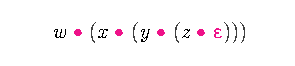
\includegraphics[draft=false,trim={25 10 25 10}]{../graphics/rhs-norm}};
      \node (rn) at ( 2, 2) {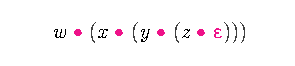
\includegraphics[draft=false,trim={25 10 25 10}]{../graphics/rhs-norm}};
      \node (la) at (-6, 0) {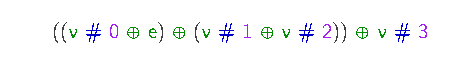
\includegraphics[draft=false,trim={25 10 22 10}]{../graphics/lhs-ast}};
      \node (ra) at ( 6, 0) {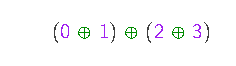
\includegraphics[draft=false,trim={25 10 48 10}]{../graphics/rhs-ast}};
      \node (le) at (-2,-2) {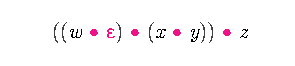
\includegraphics[draft=false,trim={25 10 23 10}]{../graphics/lhs-expr}};
      \node (re) at ( 2,-2) {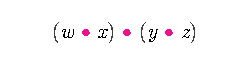
\includegraphics[draft=false,trim={25 10 20 10}]{../graphics/rhs-expr}};
      \draw[|-stealth] (la) to[out=90 , in=180] node[midway, fill=bg] {\AgdaFunction{⟦\_⇓⟧}} (ln);
      \draw[|-stealth] (la) to[out=270, in=180] node[midway, fill=bg] {\AgdaFunction{⟦\_⟧} } (le);
      \draw[|-stealth] (ra) to[out=90 , in=0  ] node[midway, fill=bg] {\AgdaFunction{⟦\_⇓⟧}} (rn);
      \draw[|-stealth] (ra) to[out=270, in=0  ] node[midway, fill=bg] {\AgdaFunction{⟦\_⟧} } (re);
      \foreach \e/\n in {le/ln,re/rn}
        \foreach \shft in {-0.6pt,0.6pt}
          \draw[AgdaField, transform canvas={xshift=\shft}, snake=coil, segment aspect=0, segment amplitude=0.4pt, segment length=4pt] (\e) -- (\n);
      \node[fill=bg] at (-2, 0) {\AgdaFunction{correct}};
      \node[fill=bg] at ( 2, 0) {\AgdaFunction{correct}};
      \foreach \shft in {-1.6pt, 0pt}
        \draw[AgdaDatatype, transform canvas={yshift=\shft}] (ln) -- (rn);
      \draw[AgdaDatatype, transform canvas={yshift=1.6pt}] (ln) -- (rn) node[midway, above] {\AgdaInductiveConstructor{refl}};
    \end{tikzpicture}
  }
\end{frame}
\begin{frame}[standout]
  Now, just to prove homomorphism!
  \note{
    I won't go through the homomorphism proofs, but effectively we need to prove
    it for each case in the expression constructor.
  }
\end{frame}
\begin{frame}
  \frametitle{Moving on to Polynomials}
  \note{
    We now know the components required for an automatic solver for some
    algebra: a canonical form, a concrete representation of expressions, and a
    proof of correctness. We now turn our focus to polynomials.

    The state-of-the art approach is presented in this paper.
  }
  \bibentry{gregoire_proving_2005}
\end{frame}
\begin{frame}
  \frametitle{Canonical Form}
  \note{
    The canonical representation of polynomials is a list of coefficients, least
    significant first (``Horner Normal Form''). Our initial attempt at encoding
    this representation is as follows.
  }
  \ExecuteMetaData[../Rings.tex]{dense-impl}
\end{frame} 
\begin{frame}
  \frametitle{Horner's Rule}
  \note<1>{
    Horner's rule is a method for evaluating polynomials which lets you avoid
    repeatedly exponentiating the input variable.
  }
  \begin{align*}
  p(x) &= a_0x^0 + a_1x^1 + a_2x^2 + ... a_nx^n \\
       &= a_0 + x(a_1 + x(a_2 + x (... a_n + x(0))))
  \end{align*}
  \pause
  \note<2>{
    Haskellers will recognize it as a foldr operation.
  }
  \ExecuteMetaData[../Rings.tex]{dense-eval}
\end{frame}
\begin{frame}
  \frametitle{Problems}
  \note<1>{As it stands, the above representation has two problems}
  \pause

  \note<2>{
    The representation suffers from the problem of trailing zeroes. In other
    words, the polynomial $2x$ could be represented by any of the following:

    This is a problem for a solver: the whole \emph{point} is that equivalent
    expressions are represented the same way. 
  }
  \begin{description}
  \item[Redundancy]
      \begin{align*}
        2x = \; & 0, 2 \\
                & 0, 2, 0 \\
                & 0, 2, 0, 0 \\
                & 0, 2, 0, 0, 0, 0, 0
      \end{align*}
      \pause
    \item[Inefficiency]
  \end{description}

  \note<3>{
    Expressions will tend to have large gaps, full only of zeroes. Something
    like $x^5$ will be represented as a list with 6 elements, only the last one
    being of interest. Since addition is linear in the length of the list, and
    multiplication quadratic, this is a major concern.
  }
\end{frame}
\begin{frame}[fragile]
  \frametitle{A Sparse Encoding}
  \note<1>{
    The solution usually used is a ``power index''. A representation of the gap
    between adjacent nonzero coefficients.

    We rewrite the following equation as so:
  }

  \(3 + 2x^2 + 4x^5 + 2x^7\) \pause \(= x^0 (3 + x x^1 (2 + x x^2 * (4 + x x^1 (2 + x 0))))\)
  \note<2>{
    And then we can represent it in a list like so:
  }

  \begin{minted}[autogobble]{Haskell}
    [(3,0),(2,1),(4,2),(2,1)]
  \end{minted}
\end{frame}
\begin{frame}
  \note{
    We actually go further than the previous approach, because we \emph{prove}
    that the coefficients are in normal form.
  }
  \ExecuteMetaData[../Rings.tex]{sparse-decl}
\end{frame}
\begin{frame}
  \frametitle{Algebra of Programming}
  \note{
    The full implementation continues like that, and we add more variables, and
    so on.

    One component of the implementation needs to prove termination, which we do
    with well-founded recursion.

    The only last thing I'll mention is with regards to the nature of the
    proofs. They use a technique called the ``algebra of programming'' to
    shorten them up: because most of our functions are defined using
    higher-order folds and so on, we can express the proofs in very abstract,
    terse terms.

    The proofs are still roughly 1000 lines long, though.
  }
  \bibentry{bird_algebra_1997}

  \bibentry{mu_algebra_2009}
\end{frame}
\begin{frame}
  \frametitle{Interface}
  \note{
    Though what we have works, it's still awkward to use, because we ask the
    user to construct the AST themselves. This means they write the type twice,
    and it is often tedious to do so.

    This is the ``automatic'' proof for the monoid solver we had previously.
  }
  \ExecuteMetaData[../Monoids.tex]{ident-auto-proof}
\end{frame}
\begin{frame}[t, fragile]
  \vspace*{2.5cm}
  \adjustbox{width=1.15\linewidth, center}{
    \begin{tikzpicture}
      % \draw[help lines] (-8,-4) grid (8,3); 
      \node (ln) at (-2, 2) {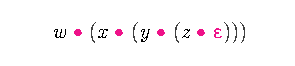
\includegraphics[draft=false,trim={25 10 25 10}]{../graphics/rhs-norm}};
      \node (rn) at ( 2, 2) {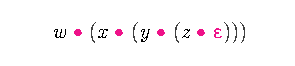
\includegraphics[draft=false,trim={25 10 25 10}]{../graphics/rhs-norm}};
      \node (la) at (-6, 0) {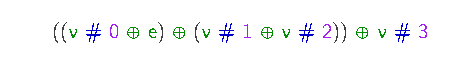
\includegraphics[draft=false,trim={25 10 22 10}]{../graphics/lhs-ast}};
      \node (ra) at ( 6, 0) {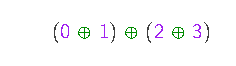
\includegraphics[draft=false,trim={25 10 48 10}]{../graphics/rhs-ast}};
      \node (le) at (-2,-2) {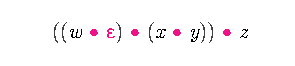
\includegraphics[draft=false,trim={25 10 23 10}]{../graphics/lhs-expr}};
      \node (re) at ( 2,-2) {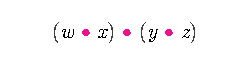
\includegraphics[draft=false,trim={25 10 20 10}]{../graphics/rhs-expr}};
      \draw[|-stealth] (la) to[out=90 , in=180] node[midway, fill=bg] {\AgdaFunction{⟦\_⇓⟧}} (ln);
      \draw[|-stealth] (la) to[out=270, in=180] node[midway, fill=bg] {\AgdaFunction{⟦\_⟧} } (le);
      \draw[|-stealth] (ra) to[out=90 , in=0  ] node[midway, fill=bg] {\AgdaFunction{⟦\_⇓⟧}} (rn);
      \draw[|-stealth] (ra) to[out=270, in=0  ] node[midway, fill=bg] {\AgdaFunction{⟦\_⟧} } (re);
      \foreach \e/\n in {le/ln,re/rn}
        \foreach \shft in {-0.6pt,0.6pt}
          \draw[AgdaField, transform canvas={xshift=\shft}, snake=coil, segment aspect=0, segment amplitude=0.4pt, segment length=4pt] (\e) -- (\n);
      \node[fill=bg] at (-2, 0) {\AgdaFunction{correct}};
      \node[fill=bg] at ( 2, 0) {\AgdaFunction{correct}};
      \foreach \shft in {-1.6pt, 0pt}
        \draw[AgdaDatatype, transform canvas={yshift=\shft}] (ln) -- (rn);
      \draw[AgdaDatatype, transform canvas={yshift=1.6pt}] (ln) -- (rn) node[midway, above] {\AgdaInductiveConstructor{refl}};
      \draw<2>[-angle 90, dashed] (re) to[out=270, in=270] node[near start, fill=bg] {\AgdaKeyword{quoteTerm}} ([shift={(1,0)}]ra.south);
      \draw<2>[-angle 90, dashed] (le) to[out=270, in=270] node[near start, fill=bg] {\AgdaKeyword{quoteTerm}} ([shift={(-1,0)}]la.south);
    \end{tikzpicture}
  }
  \note<1>{
    What we'd like to do is provide the ASTs here automatically, from the two
    expressions at the bottom.
  }
  \note<2>{
    What can we use for that? \emph{Reflection}

    Reflection is often thought to be the purview of unsafe or dynamic
    languages, but it actually fits really well into the dependently typed
    setting. As it happens, Agda has a decent (type-directed) macro system. The
    end result is a very clean system
  }
\end{frame}
\begin{frame}[standout]
  The Finished Solver
\end{frame}
\begin{frame}
  \note{
    Even more, because this relies on the \emph{type} of the hole (the inferred
    obligation) if you need to prove two things line up, you just pinpoint where
    they son't match, and say ``solve, please!''
  }
  \ExecuteMetaData[../ReflectDemo.tex]{refl-lemma}
\end{frame}
\begin{frame}[fragile]
  \frametitle{Setoids}
  \note<1>{
    We used a setoid throughout the solver, which really made things difficult
    for us.

    Usually, The purpose of this particular hair shirt is flexibility: users can
    still use the solver even if their type only satisfies the monoid laws
    modulo some equivalence relation (perhaps they are have an implementation of
    finite, mergeable sets as balanced trees, and want to treat two sets as
    equivalent if their elements are equal, even if their internal structures
    are not).

    It also frees up some very interesting applications, though.
  }
  \note<2>{
    All you need a setoid to be is something with symmetry, reflexivity, and
    transitivity. One example would be a list of rewrite rules! Now, the output
    is a proof, along with a \emph{step-by-step} solution to how you got from
    one equation to the other. We get wolfram alpha for free! And it's verified!

    Reflexivity is the empty list.

    Transitivity is concatenation.

    Symmetry is reverse.
  }
  \pause

  \only<2>{
    \begin{block}{Pedagogical Solutions}
      \ExecuteMetaData[BasicTypes.tex]{traced}
    \end{block}
  }

  \only<3>{
    \begin{block}{Isomorphisms}
      \ExecuteMetaData[BasicTypes.tex]{iso}
    \end{block}
  }
  \note<3>{
    Some of the type operations we mentioned earlier were ring-like: sum types,
    product types, the empty type, the singleton type, etc.

    Turns out these can be directly translated into polynomials!

    And the equivalence relation? An isomorphism! So now we can automatically
    construct isomorphisms between equivalent types.
  }
\end{frame}
\begin{frame}[fragile]
  \frametitle{The Correct-by-Construction Approach}
  \note<1>{
    The Agda and Coq communities exhibit something of a cultural difference when it
    comes to proving things. Coq users seem to prefer writing simpler, almost
    non-dependent code and algorithms, to separately prove properties about that
    code in auxiliary lemmas. Agda users, on the other hand, seem to prefer baking
    the properties into the definition of the types themselves, and writing the
    functions in such a way that they prove those properties as they go (the
    ``correct-by-construction'' approach).

    There are advantages and disadvantages to each approach. The Coq approach, for
    instance, allows you to reuse the same functions in different settings,
    verifying different properties about them depending on what's required. In Agda,
    this is more difficult: you usually need a new type for every invariant you
    maintain (lists, and then length-indexed lists, and then sorted lists, etc.). On
    the other hand, the proofs themselves often contain a lot of duplication of the
    logic in the implementation: in the Agda style, you avoid this duplication, by
    doing both at once. Also worth noting is that occasionally attempting to write a
    function that is correct by construction will lead to a much more elegant
    formulation of the original algorithm, or expose symmetries between the proof
    and implementation that would have been difficult to see otherwise.
  }
  \note<2>{
    The gregoire version as an example, is very much in the Coq style: the
    definition of the polynomial type has no type indices, and makes no requirements
    on its internal structure:

    The implementation presented here straddles both camps: we verify
    homomorphism in separate lemmas, but the type itself does carry information:
    it's indexed by the number of variables it contains, for instance, and it
    statically ensures it's always in canonical form. 
  }
  \begin{onlyenv}<2>
    \bibentry{gregoire_proving_2005}

    \begin{minted}[autogobble]{Coq}
      Inductive Pol (C:Set) : Set :=
        | Pc : C -> Pol C
        | Pinj : positive -> Pol C -> Pol C
        | PX : Pol C -> positive -> Pol C -> Pol C.
    \end{minted}
  \end{onlyenv} 

  \only<3>{\bibentry{geuvers_automatically_2017}}
  \note<3>{
    The correct-by-construction approach is explored in Idris, but they don't
    employ the same level of reflection or optimisation as we do.
  }
  \only<4>{\ExecuteMetaData[../Constr.tex]{constr-def}}
  \note<4>{
    Nonetheless, we do provide an implementation of this version, for
    comparison.
  }
\end{frame}
\section{The \(p\)-Adics}
\end{document}
